%%%%%%%%%%%%%%%%%%%%%%%%%%%%%%%%%%%%%%%%%
\documentclass[11pt]{report}
\usepackage{graphics}
\usepackage{graphicx}
\usepackage{epsfig}
\usepackage{fancyhdr}
\usepackage{fullpage}
\usepackage{amsmath}
\usepackage{flexisym}
\usepackage{caption}
\usepackage{subcaption}
\usepackage{algpseudocode,algorithm}
\usepackage[section]{placeins}
\usepackage{amssymb}
\usepackage{textcomp}
\usepackage{tocloft}
\usepackage{multicol}
\usepackage{acronym}
\usepackage{setspace}
\usepackage{enumitem}
\usepackage{hyperref}
\usepackage{acro}
\usepackage{booktabs}
\usepackage{float}
\usepackage{xcolor}
\usepackage{colortbl}
\usepackage{adjustbox}

% Define \changefont for use in headers
\newcommand{\changefont}{\fontsize{9}{11}\selectfont}

\onehalfspacing

\newlength{\mylen}
\renewcommand{\cftfigpresnum}{\figurename\enspace}
\renewcommand{\cftfigaftersnum}{:}
\settowidth{\mylen}{\cftfigpresnum\cftfigaftersnum}
\addtolength{\cftfignumwidth}{\mylen}

\renewcommand{\cfttabpresnum}{\tablename\enspace}
\renewcommand{\cfttabaftersnum}{:}
\settowidth{\mylen}{\cfttabpresnum\cfttabaftersnum}
\addtolength{\cfttabnumwidth}{\mylen}


\begin{document}
\renewcommand\bibname{References}
\pagestyle{fancy}
\fancyhead{}
\fancyfoot{}
\fancyfoot[c]{\thepage}
\fancyfoot[l]{\footnotesize B.Tech CSE(AI) 2024-2028}
%\lhead{abcd}
\renewcommand{\chaptermark}[1]{
\markboth{\thechapter.\ #1}{}}
\renewcommand{\headrulewidth}{0.1pt}
\fancyhead[r]{\slshape \leftmark}
\addtolength{\headheight}{\baselineskip}
\addtolength{\headsep}{.1in}
\lhead{\nouppercase{\rightmark}}
\rhead{\footnotesize{\nouppercase{\leftmark}}}
%\lhead{\footnotesize Project title} % use any short form if title is lengthy

\begin{titlepage}
\begin{center}

\LARGE{\textbf{IMPROVING PIPELINE EFFICIENCY THROUGH INSTRUCTION REORDERING}}\\

\vspace{0.3in}
\large{\textbf{ MICRO PROJECT REPORT  \\}}
\large{\textbf{ PBCST404 - COMPUTER ORGANIZATION AND ARCHITECTURE  \\}}
\vspace{0.3in}

\textit{Micro Project Report submitted in partial fulfillment for the degree  \\
of\\
B.Tech Computer Science \& Engineering (Artificial Intelligence)} \\[2cm]

Submitted by\\[0.5cm]

\textsc{\textbf{ANAGHA A  (Reg No: MUT24CA014)}}\\ %team member 1
\textsc{\textbf{DEON SHAJI (Reg No: MUT24CA033)}}\\
\textsc{\textbf{JOHN VARGHESE NETTADY (Reg No: MUT24CA044)}}\\
\textsc{\textbf{MERIN REJI (Reg No: MUT24CA051)}}\\


\vspace{0.2in}
\begin{figure}[h]
\begin{center}

\includegraphics[width=5.5cm]{images/Mits logo.jpg}
\end{center}
\end{figure}
\vspace{-0.8cm}
\textsc{\textbf{DEPARTMENT OF ARTIFICIAL INTELLIGENCE AND DATA SCIENCE}}\\[0.10cm]
%\includegraphics[width=9cm]{mits_logo.jpg}\\
\textit{(Affiliated to APJ Abdul Kalam Technological University)}\\
\vspace{0.2in}
{\upshape \textbf{March  2026}} % mention the month of your presentation.
\end{center}
\end{titlepage}



\begin{titlepage}
\begin{figure}[h]
\begin{center}

\includegraphics[width=0.30\textwidth]{images//Mits logo.jpg}\par\vspace{0.1cm}
\end{center}
\end{figure}
\begin{center}
\vspace{-2cm}
\text{\normalsize \textbf{ Varikoli P.O., Puthencruz-682308}}\\[0.5cm]

\textsc{\textbf{\large{DEPARTMENT OF ARTIFICIAL INTELLIGENCE AND DATA SCIENCE}}}\\[0.4cm]
\vspace{0.5cm}
\begin{center}
   {\scshape \Large \bfseries CERTIFICATE \par}
\end{center}


\end{center}
This is to certify that the micro project report entitled \textbf{``IMPROVING PIPELINE EFFICIENCY THROUGH INSTRUCTION REORDERING``} submitted by \textbf{ANAGHA A (Reg No: MUT24CA014), DEON SHAJI (Reg No: MUT24CA033), JOHN VARGHESE NETTADY  (Reg No: MUT24CA044), MERIN REJI (Reg No: MUT24CA051)} of Semester IV is a bonafide account of the work done by them under my supervision during the academic year 2025-26.\\[0.7cm]

\vspace{1.5cm}

\begin{flushleft}
Dr.\ Parvathy Jyothi\\
Faculty-in-Charge
\end{flushleft}

\vspace{1cm}

{\noindent Place: \newline \noindent Date:}

\vspace{1cm}



\end{titlepage}



\newpage

\pagenumbering{roman}
\setcounter{page}{2}
\thispagestyle{plain}
\begin{center}
\section*{ABSTRACT}
\end{center}
\addcontentsline{toc}{section}{\uppercase\textbf{Abstract}}

Instruction reordering is a useful technique that helps improve the performance of pipelined processors. In a pipelined system, instructions are executed in stages, but sometimes one instruction depends on the result of a previous one. This creates delays called pipeline stalls, which slow down the overall execution.

In this project, we explore how rearranging instructions can reduce these delays. Six benchmark C programs --- Bubble Sort, Convolution, Fibonacci, Matrix Multiplication, Perfect Number, and Transpose --- are compiled to RISC-V assembly and then reordered using a sliding-window Python scheduler (window size~3). Both the original and reordered versions are executed using the Ripes RISC-V pipeline simulator, under two hardware configurations: a pipeline with hardware data-forwarding and one without.

We compare the performance of both versions using metrics such as cycle count, CPI (Cycles Per Instruction), pipeline efficiency, and stall count. Across all six benchmarks, instruction reordering reduced CPI by \textbf{3.77\%} and stall cycles by \textbf{8.08\%}, saving a total of \textbf{21,114 clock cycles}. The Fibonacci benchmark achieved the highest stall reduction of \textbf{28.08\%} and a speedup of \textbf{1.061$\times$}, while all programs maintained full semantic correctness verified by register-state comparison.

Overall, this project provides a better understanding of pipeline hazards, instruction dependencies, and how simple software-level optimization techniques can improve processor performance without any hardware modification.


\newpage
\pagenumbering{roman}
\setcounter{page}{3}
\thispagestyle{plain}
\begin{center}
\textbf{\large CO -- PO / PSO ARTICULATION MATRIX }
\end{center}

\vspace{0.5cm}
\noindent
CO1: Identify the basic structure and functional units of a digital computer and the features of RISC architecture
\newline
\noindent
CO2: Experiment with the single cycle processor, pipelining, and the associated problems.
\newline
\noindent
CO3: Utilize the memory organization in modern computer systems.
\newline
\noindent
CO4: Experiment with the I/O organization of a digital computer.
\vspace{0.5cm}

\textbf{NB: Adjust the dimension of the below tables. The tables of CO-PO -PSO mapping and SDG must follow same dimension}


\begin{table}[h!]
\centering
\caption{CO--PO/PSO Articulation Matrix}
\label{tab:copo}
\renewcommand{\arraystretch}{1.0}
\resizebox{\textwidth}{!}{
\begin{tabular}{|c|*{11}{c|}*{2}{c|}}
\hline
\textbf{Course Outcome} & \multicolumn{11}{c|}{\textbf{Program Outcome (PO)}} & \multicolumn{2}{c|}{\textbf{PSO}} \\
\cline{2-14}
 & 1 & 2 & 3 & 4 & 5 & 6 & 7 & 8 & 9 & 10 & 11 & 1 & 2 \\
\hline

CO1 & 3 & 3 & 3 &  & 3 &  &  & 3 & 3 &  & 3 & 1 & 2 \\
\hline

CO2 & 3 & 3 & 3 & 3 & 3 &  &  & 3 & 3 &  & 3 & 2 & 3 \\
\hline

CO3 & 3 & 3 & 3 & 3 & 3 &  &  & 3 & 3 &  & 3 & 1 & 3 \\
\hline

CO4 & 3 & 3 & 3 & 3 & 3 &  &  & 3 & 3 &  & 3 & 1 & 3 \\
\hline

\end{tabular}
}
\end{table}

\vspace{0.7cm}

\begin{center}
\textbf{\large SUSTAINABLE DEVELOPMENT GOALS (SDG) ADDRESSED}
\end{center}

\vspace{0.3cm}

\begin{table}[h!]
\centering
\caption{Sustainable Development Goals Addressed}
\label{tab:sdg}
\renewcommand{\arraystretch}{1.3}
\begin{tabular}{|c|c|p{6.2cm}|}
\hline
\textbf{SDG} & \textbf{Target} & \textbf{Justification} \\
\hline

9 & Optimize processor performance by reducing pipeline stalls. &
Improves system efficiency and supports advanced computing infrastructure.  \\
\hline

\end{tabular}
\end{table}


\newpage
\tableofcontents

\newpage
\renewcommand\thepage{\arabic{page}}

\clearpage

\setlength{\headheight}{15pt}

\pagestyle{fancy}
\fancyhf{}
\lhead{\changefont\leftmark}
\rhead{\changefont\rightmark}
\cfoot{\thepage}
\renewcommand{\chaptermark}[1]{%
\markboth{#1}{}}
\renewcommand{\sectionmark}[1]{%c
\markright{#1}{}}
\renewcommand{\headrulewidth}{0.5pt}

\pagenumbering{arabic}
\setcounter{page}{1}
\chapter{INTRODUCTION}
\vspace{-1 cm}

\section{PROBLEM STATEMENT}
\noindent
To analyze the effect of instruction reordering on pipeline performance in a pipelined processor and study how reordering instructions can reduce pipeline stalls and improve overall execution efficiency.

\vspace{0.3cm}
Pipelining is a widely used technique in modern processors to increase instruction throughput by executing multiple instructions simultaneously. It divides the execution process into different stages such as instruction fetch, decode, execute, memory access, and write back. While pipelining improves performance, it also introduces certain challenges.

One of the major challenges is the occurrence of pipeline hazards. These hazards arise when instructions depend on the results of previous instructions. Among these, data hazards are the most common, especially the Read After Write (RAW) dependency. A typical example is the load-use hazard, where a value loaded from memory is immediately required by the next instruction.

In such situations, the processor cannot proceed with execution immediately and must wait for the data to become available. This delay results in pipeline stalls, where some stages of the pipeline remain idle. These stalls increase the total execution time and reduce the efficiency of the processor.

To overcome this issue, instruction reordering is used as an optimization technique. In instruction reordering, independent instructions are rearranged in such a way that they fill the delay slots between dependent instructions. This allows the pipeline to remain active and reduces idle cycles.

However, reordering must be done carefully to preserve program correctness. The key constraint is the Read After Write (RAW) dependency: a later instruction that reads a register whose value has not yet been written back by an earlier instruction must always execute after its producer.

In this project, we analyze how instruction reordering affects pipeline performance. Assembly programs are examined and reordered using Python-based approaches. The performance of both original and reordered programs is then evaluated using the Ripes simulator.
By comparing cycle count, CPI, and IPC, the impact of instruction reordering on performance is analyzed.

\section{OBJECTIVES}
\noindent

\textbf{Understanding Pipeline Architecture}

\begin{itemize}
\item \textbf{Study of Pipeline Stages} \\
Understand the five stages of pipelining: Instruction Fetch (IF), Instruction Decode (ID), Execute (EX), Memory Access (MEM), and Write Back (WB). Each stage performs a specific task, and instructions move sequentially through these stages during execution.

\item \textbf{Overlapping Execution} \\
Learn how multiple instructions are processed simultaneously in different stages of the pipeline. This overlapping of instructions increases throughput and improves overall processor performance compared to non-pipelined systems.

\item \textbf{Pipeline Hazards} \\
Identify different types of hazards such as data hazards, structural hazards, and control hazards. Study how these hazards affect smooth execution and reduce efficiency.
\end{itemize}

\vspace{0.7cm}

\noindent
\textbf{Analysing Instruction Dependencies}

\begin{itemize}
\item \textbf{Read After Write (RAW) Dependencies} \\
Examine how RAW data dependencies arise: a later instruction needs a register value that an immediately preceding instruction has not yet written back. RAW is the dominant hazard type in RISC-V in-order pipelines and the primary target of instruction reordering.

\item \textbf{Impact on Pipeline Execution} \\
Analyze how dependencies create pipeline hazards and lead to stalls or bubble cycles. These stalls increase execution time and reduce processor efficiency.

\item \textbf{Stall Analysis} \\
Study how the processor handles dependencies by inserting stalls. Understand how these stalls affect performance metrics like cycle count and CPI.
\end{itemize}

\vspace{0.7cm}

\noindent
\textbf{Applying Reordering and Evaluating Performance}

\begin{itemize}
\item \textbf{Instruction Reordering Technique} \\
Apply instruction reordering by rearranging independent instructions between dependent ones. This helps in reducing pipeline stalls and improving instruction flow.

\item \textbf{Maintaining Correctness} \\
Ensure that reordering does not introduce new RAW hazards among the rearranged instructions. The program output must remain identical before and after reordering, verified by comparing final register states.

\item \textbf{Performance Evaluation} \\
Compare the performance of original and reordered programs using metrics such as cycle count, CPI (Cycles Per Instruction), and IPC (Instructions Per Cycle). Analyze how reordering improves execution efficiency.
\end{itemize}

% ============================================================
\chapter{SIMULATOR}
% ============================================================

\section{INTRODUCTION TO SIMULATOR}

The Ripes RISC-V pipeline simulator is an open-source, visual, graphical tool designed for educational exploration of processor pipeline behavior. Ripes accepts standard RISC-V assembly (\texttt{.s}) files and executes them cycle-by-cycle through a configurable in-order pipeline, exposing every internal signal at each stage.

For this project, Ripes is configured to model a \textbf{classic 5-stage in-order pipeline}: Instruction Fetch (IF) $\rightarrow$ Instruction Decode (ID) $\rightarrow$ Execute (EX) $\rightarrow$ Memory Access (MEM) $\rightarrow$ Write Back (WB). Two hardware configurations are evaluated:

\begin{enumerate}
    \item \textbf{With Data Forwarding} --- the pipeline includes bypass paths (EX$\rightarrow$EX and MEM$\rightarrow$EX) that allow computed values to be routed directly to dependent instructions, drastically reducing stalls.
    \item \textbf{Without Data Forwarding} --- no bypass paths exist; the pipeline must stall for two cycles on every RAW hazard, giving worst-case stall counts that highlight the full benefit of reordering.
\end{enumerate}

After execution, Ripes outputs a JSON file capturing total cycle count, instruction count, stall breakdown, and final register state. These JSON files are parsed by the \texttt{analyse\_results.py} script to compute all performance metrics.

\section{WORKING OF SIMULATOR}

\subsection{Loading and Running Assembly Programs}

The workflow for using Ripes in this project is automated via the Python script \texttt{run\_benchmarks.py}. This script invokes Ripes in \textit{headless} (CLI) mode for each benchmark in both its original and reordered forms under both hardware configurations. The general steps are:

\begin{enumerate}
    \item \textbf{Program Loading:} Each \texttt{.s} file is loaded into Ripes using its CLI interface. The memory layout is configured with a default instruction memory region.
    \item \textbf{Simulation:} Ripes steps through the program cycle by cycle until the program terminates via an \texttt{ecall} (system call with \texttt{a7 = 10}).
    \item \textbf{Result Export:} On termination, Ripes writes a JSON output file containing the pipeline statistics and final register state.
    \item \textbf{Post-Processing:} The JSON file is parsed by \texttt{analyse\_results.py} to extract cycle count, instruction count, CPI, stall cycles, and pipeline efficiency.
\end{enumerate}

% -------------------------------------------------------
% [PLACEHOLDER IMAGE 1]
% ADD: A screenshot of the Ripes simulator UI showing a loaded
%      RISC-V assembly program in the pipeline view, with the
%      five pipeline stage registers (IF/ID/EX/MEM/WB) visible.
%      Suggested file: report/ripes_pipeline_view.png
% -------------------------------------------------------
\begin{figure}[H]
    \centering
    \includegraphics[width=0.9\textwidth]{placeholder_ripes_ui}
    \caption{Ripes Simulator --- 5-stage pipeline view with a loaded RISC-V assembly program}
    \label{fig:ripes_ui}
\end{figure}

\subsection{Memory Configuration}

The simulator's memory is configured to provide a flat address space suitable for the benchmark programs. The stack pointer is initialised to a high address so that array-based programs (e.g., Bubble Sort, Matrix Multiplication) have sufficient space for their working data.

% -------------------------------------------------------
% [PLACEHOLDER IMAGE 2]
% ADD: A screenshot of the Ripes memory/register configuration
%      dialog, showing the stack pointer initial value and
%      memory region settings.
%      Suggested file: report/ripes_memory_config.png
% -------------------------------------------------------
\begin{figure}[H]
    \centering
    \includegraphics[width=0.75\textwidth]{placeholder_ripes_memory_config}
    \caption{Memory configuration settings in Ripes}
    \label{fig:ripes_memory_config}
\end{figure}

\subsection{Forwarding vs.\ No-Forwarding Mode}

Ripes allows toggling hardware data forwarding on or off via its pipeline settings. Figure~\ref{fig:ripes_forwarding} illustrates the forwarding configuration panel. Disabling forwarding forces the pipeline to insert two stall cycles for each RAW hazard, dramatically increasing the total cycle count and making the effect of software reordering much more visible.

% -------------------------------------------------------
% [PLACEHOLDER IMAGE 3]
% ADD: A screenshot of the Ripes pipeline settings dialog
%      showing the "Enable forwarding" checkbox or toggle.
%      Suggested file: report/ripes_forwarding_toggle.png
% -------------------------------------------------------
\begin{figure}[H]
    \centering
    \includegraphics[width=0.6\textwidth]{placeholder_ripes_forwarding_toggle}
    \caption{Forwarding enable/disable setting in Ripes pipeline configuration}
    \label{fig:ripes_forwarding}
\end{figure}

\subsection{System Architecture and Toolchain Workflow}

The proposed toolchain is built as a modular Python-based framework. It handles everything from compiling high-level C code to evaluating the final reordered assembly in the Ripes simulator.

\subsubsection{Project Structure}
The repository is systematically organized to separate source scripts, generated assemblies, and test outputs.

\begin{verbatim}
.
├── riscv_parser.py           # Reusable parser and instruction metadata extractor
├── riscv_reorder_minimal.py  # Sliding-window reorder pass logic
├── reorder_all.py            # Batch-reorder script for entire directories
├── run_benchmarks.py         # Automates execution and JSON collection in Ripes
├── analyse_results.py        # Parses JSON results to generate CSV analysis
├── run.py                    # Top-level coordinator runner
├── compile_c_for_ripes.py    # Compiles C programs to raw GCC assembly
├── convert_for_ripes.py      # Cleans and formats assembly strictly for Ripes
└── verify_results.py         # Validates semantic correctness via register matching
\end{verbatim}

\subsubsection{Compilation and Conversion Pipeline}

Figure~\ref{fig:c_to_asm_flow} illustrates the full path from a C source file to a Ripes-ready reordered assembly file. The four principal stages are:

\begin{enumerate}
    \item \textbf{C Compilation (\texttt{compile\_c\_for\_ripes.py} / GCC):} Each \texttt{.c} file in the \texttt{programs/} directory is compiled with \texttt{riscv32-unknown-elf-gcc -march=rv32i -mabi=ilp32 -O0 -nostdlib -S} to produce a raw GCC \texttt{.s} file. The \texttt{-O0} flag disables compiler optimisations, producing a naive baseline assembly that closely mirrors the C source and retains all natural RAW hazard opportunities.
    \item \textbf{Ripes Conversion (\texttt{convert\_for\_ripes.py}):} The raw GCC output contains directives that Ripes cannot parse (e.g.\ \texttt{.file}, \texttt{.option}, \texttt{.attribute}, \texttt{.type}, \texttt{.size}). This script strips those unsupported directives, inlines the \texttt{\_\_mulsi3} software-multiply helper if required, and prepends a \texttt{\_start} stub that calls \texttt{main} then issues \texttt{ecall} with \texttt{a7~=~10} to terminate the Ripes simulation cleanly. The result is a \texttt{*\_ripes.s} file.
    \item \textbf{Instruction Reordering (\texttt{riscv\_reorder\_minimal.py}):} The cleaned assembly file is fed through the sliding-window scheduler (window size~3). The scheduler scans instruction pairs and, upon detecting a RAW hazard, searches the next two positions for an independent instruction to promote. Both the original and reordered \texttt{.s} files are kept as separate outputs.
    \item \textbf{Ripes Simulation via CLI (\texttt{run\_benchmarks.py}):} Both the original and reordered files are executed by \texttt{run\_benchmarks.py} through the Ripes headless CLI under two pipeline configurations (forwarding enabled and disabled), producing four JSON output files per benchmark.
\end{enumerate}

\begin{figure}[H]
    \centering
    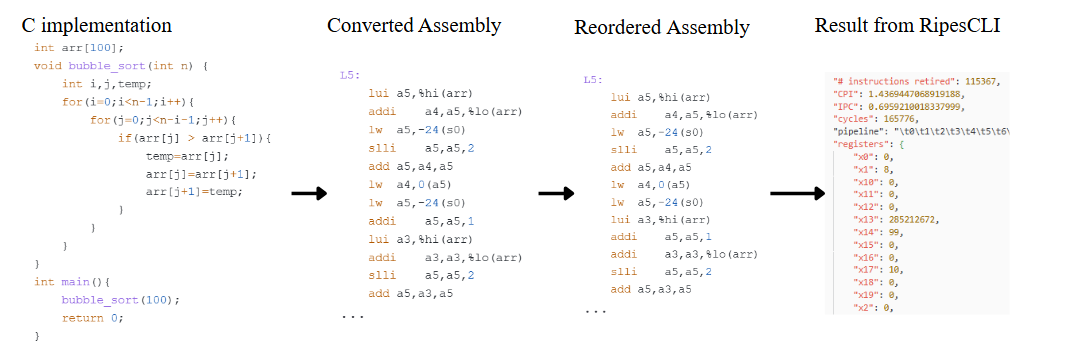
\includegraphics[width=\textwidth, height=0.42\textheight, keepaspectratio]{../images/conversion}
    \caption{Compilation and Conversion Pipeline: from C source to Ripes-ready reordered assembly}
    \label{fig:c_to_asm_flow}
\end{figure}

\subsubsection{Testing and Execution Workflow}

Once the assembly files have been compiled and converted, the evaluation pipeline shown in Figure~\ref{fig:testing_workflow} orchestrates the full benchmarking cycle. Each numbered stage below corresponds to a box in the diagram:

\begin{enumerate}
    \item \textbf{Batch Reordering (\texttt{reorder\_all.py}):} Iterates over every \texttt{.s} file in the \texttt{test scripts/} directory, applies \texttt{riscv\_reorder\_minimal.py} to each, and writes the reordered outputs to \texttt{reordered\_tests/}.
    \item \textbf{Benchmark Execution (\texttt{run\_benchmarks.py}):} Invokes Ripes in headless CLI mode for each benchmark (original and reordered) under both forwarding configurations. Four JSON result files are produced per benchmark: \texttt{<name>\_original.json}, \texttt{<name>\_reordered.json}, and their \texttt{\_no\_fw} counterparts.
    \item \textbf{Result Analysis (\texttt{analyse\_results.py}):} Reads each JSON pair, computes derived metrics (CPI, IPC, stall rate, pipeline efficiency, cycle savings, percentage improvements), and writes \texttt{analysis.csv} and \texttt{analysis\_no\_fw.csv}.
    \item \textbf{Semantic Verification (\texttt{verify\_results.py}):} Extracts the final register file state from each original/reordered JSON pair and compares them field-by-field. Any mismatch triggers a FAIL report. All six benchmarks passed this check, confirming zero correctness regressions.
    \item \textbf{Graph Generation (\texttt{build\_graphs.py}):} Reads the CSV files and produces a full suite of comparative bar charts (stall counts, stall rates, CPI, cycles, percentage improvements) saved as PNG files to \texttt{results/graphs/}.
\end{enumerate}

\begin{figure}[H]
    \centering
    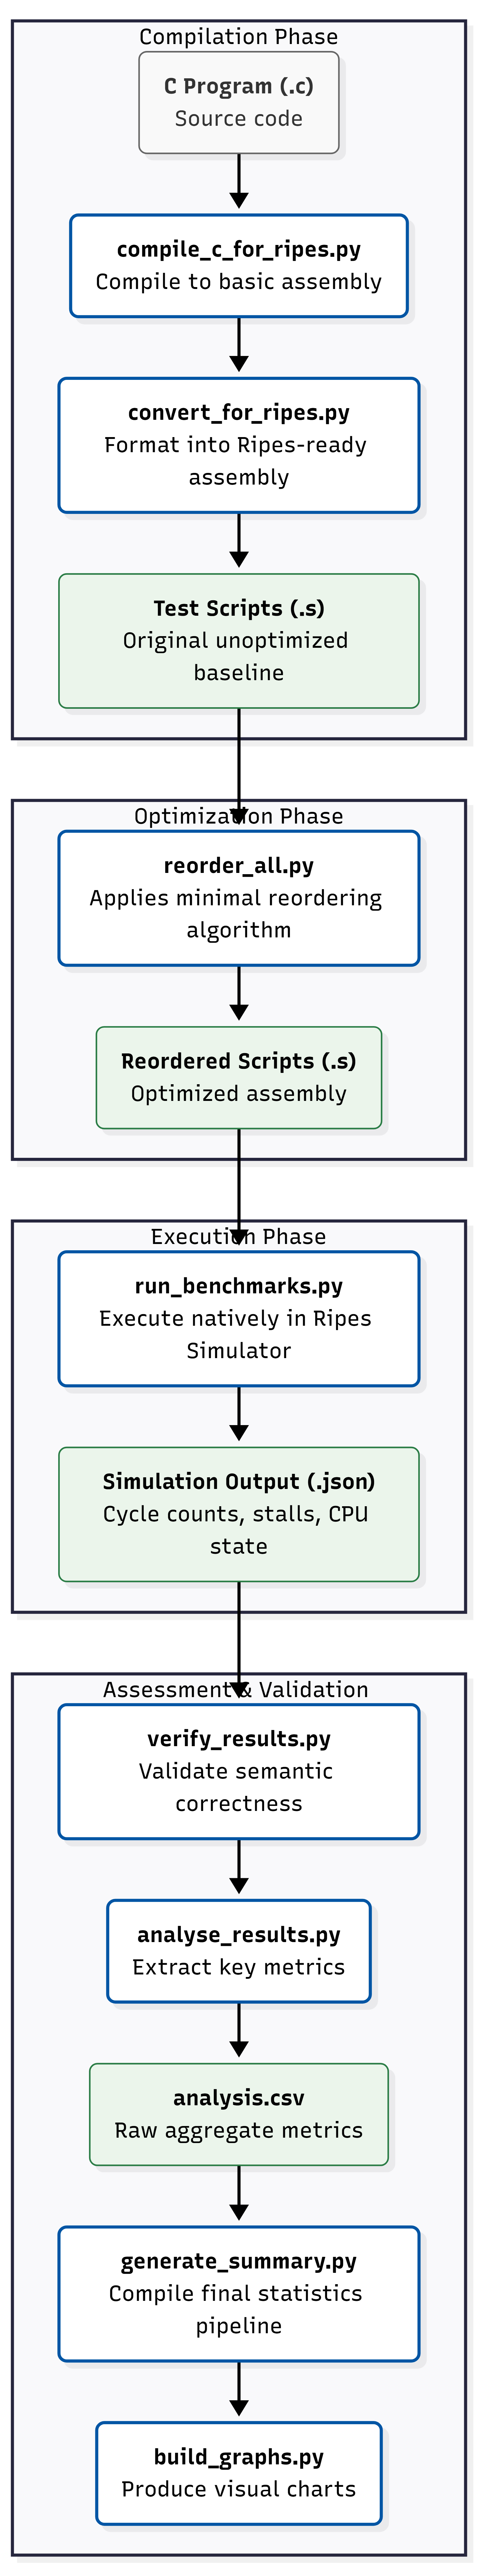
\includegraphics[width=0.24\textwidth]{../images/testing-flow}
    \caption{Testing and evaluation workflow: from assembly generation to graphical analysis}
    \label{fig:testing_workflow}
\end{figure}

% Hazard demonstration and reordering algorithm have been moved to
% Chapter 3, Section: Theoretical Background.

% ============================================================
\newpage
\chapter{PROPOSED SYSTEM}
% ============================================================

The proposed system introduces an optimization toolchain designed for textual RISC-V assembly, specifically targeting a classic in-order 5-stage pipeline (\texttt{IF $\rightarrow$ ID $\rightarrow$ EX $\rightarrow$ MEM $\rightarrow$ WB}). Its primary goal is to minimize pipeline stalls caused predominantly by Read After Write (RAW) data hazards. It intelligently reorders instructions without altering the program's intended semantic behavior.

The toolchain operates by first parsing the assembly code to extract metadata for each instruction, identifying register dependencies and memory operations. It then applies a conservative, sliding-window scheduling algorithm (window size of 3). Whenever a data dependency is detected between an instruction and its immediate predecessor, the algorithm scans the closely following instructions for a candidate that is completely independent. If an independent candidate is found, it is shifted upward between the dependent pair, effectively filling the hazard delay slot and eliminating the need for a pipeline stall. The performance impact of this static reordering is thoroughly evaluated by executing both original and reordered assemblies on the Ripes processor simulator.

\noindent
\vspace{-1 cm}
\noindent

\section{THEORETICAL BACKGROUND}

In pipelined processors, instructions undergo multiple execution phases simultaneously. While this significantly increases throughput, it also introduces the possibility of data hazards. A \textbf{Read After Write (RAW)} hazard occurs when an instruction needs a register value that has not yet been written back by an earlier instruction. To resolve this without hardware forwarding, the pipeline inserts ``bubble'' stall cycles, directly decreasing the Instructions Per Cycle (IPC) and increasing the Cycles Per Instruction (CPI).

\subsection{RAW Hazard Demonstration}

Consider the following three-instruction RISC-V sequence:

\begin{verbatim}
add x1, x2, x3   ; Instruction 1: Writes result into x1
sub x4, x1, x5   ; Instruction 2: Reads x1  <-- RAW hazard on x1
addi x6, x7, 10  ; Instruction 3: Reads x7, x0 (independent)
\end{verbatim}

\textbf{Instruction 2} depends on \textbf{Instruction 1}: it reads \texttt{x1} before \texttt{add} has completed the Write-Back stage. Without forwarding, the pipeline must stall for two cycles. \textbf{Instruction 3}, however, uses entirely different registers and has no dependency on either Instruction~1 or~2. The sliding-window scheduler detects this and promotes Instruction~3 between Instruction~1 and~2:

\begin{verbatim}
add  x1, x2, x3   ; (original position -- produces x1)
addi x6, x7, 10   ; promoted independent instruction fills the slot
sub  x4, x1, x5   ; x1 is now ready -- stall eliminated
\end{verbatim}

This single reordering eliminates the stall without changing the program's final result.

\subsection{Sliding-Window Reordering Algorithm}

The scheduling routine implemented in \texttt{riscv\_reorder\_minimal.py} applies a deterministic window of size~3 to evaluate RAW dependencies. The algorithm is:

\begin{algorithm}[H]
\caption{Window-3 RAW-Aware Reordering Algorithm}
\begin{algorithmic}[1]
\State $\text{window\_size} \gets 3$
\For{each instruction $i$ in basic block}
    \State $\text{prev} \gets \text{instruction}_{i-1}$; \quad $\text{curr} \gets \text{instruction}_{i}$
    \If{$\text{RAW\_depends\_on}(\text{prev},\ \text{curr})$}
        \State $\text{limit} \gets \min(i + \text{window\_size} - 2,\ |\text{block}| - 1)$
        \For{$j \gets i+1$ \textbf{to} limit}
            \If{$\text{candidate}_{j}$ independent of both prev and curr}
                \State Promote $\text{candidate}_{j}$ to position $i$; shift others down
                \State \textbf{break}
            \EndIf
        \EndFor
    \EndIf
\EndFor
\end{algorithmic}
\end{algorithm}

The scheduler never moves instructions across labels, branches, calls, returns, or barrier instructions (\texttt{ecall}/\texttt{ebreak}/\texttt{fence}), ensuring that scheduling regions remain semantically self-contained.

\begin{figure}[H]
    \centering
    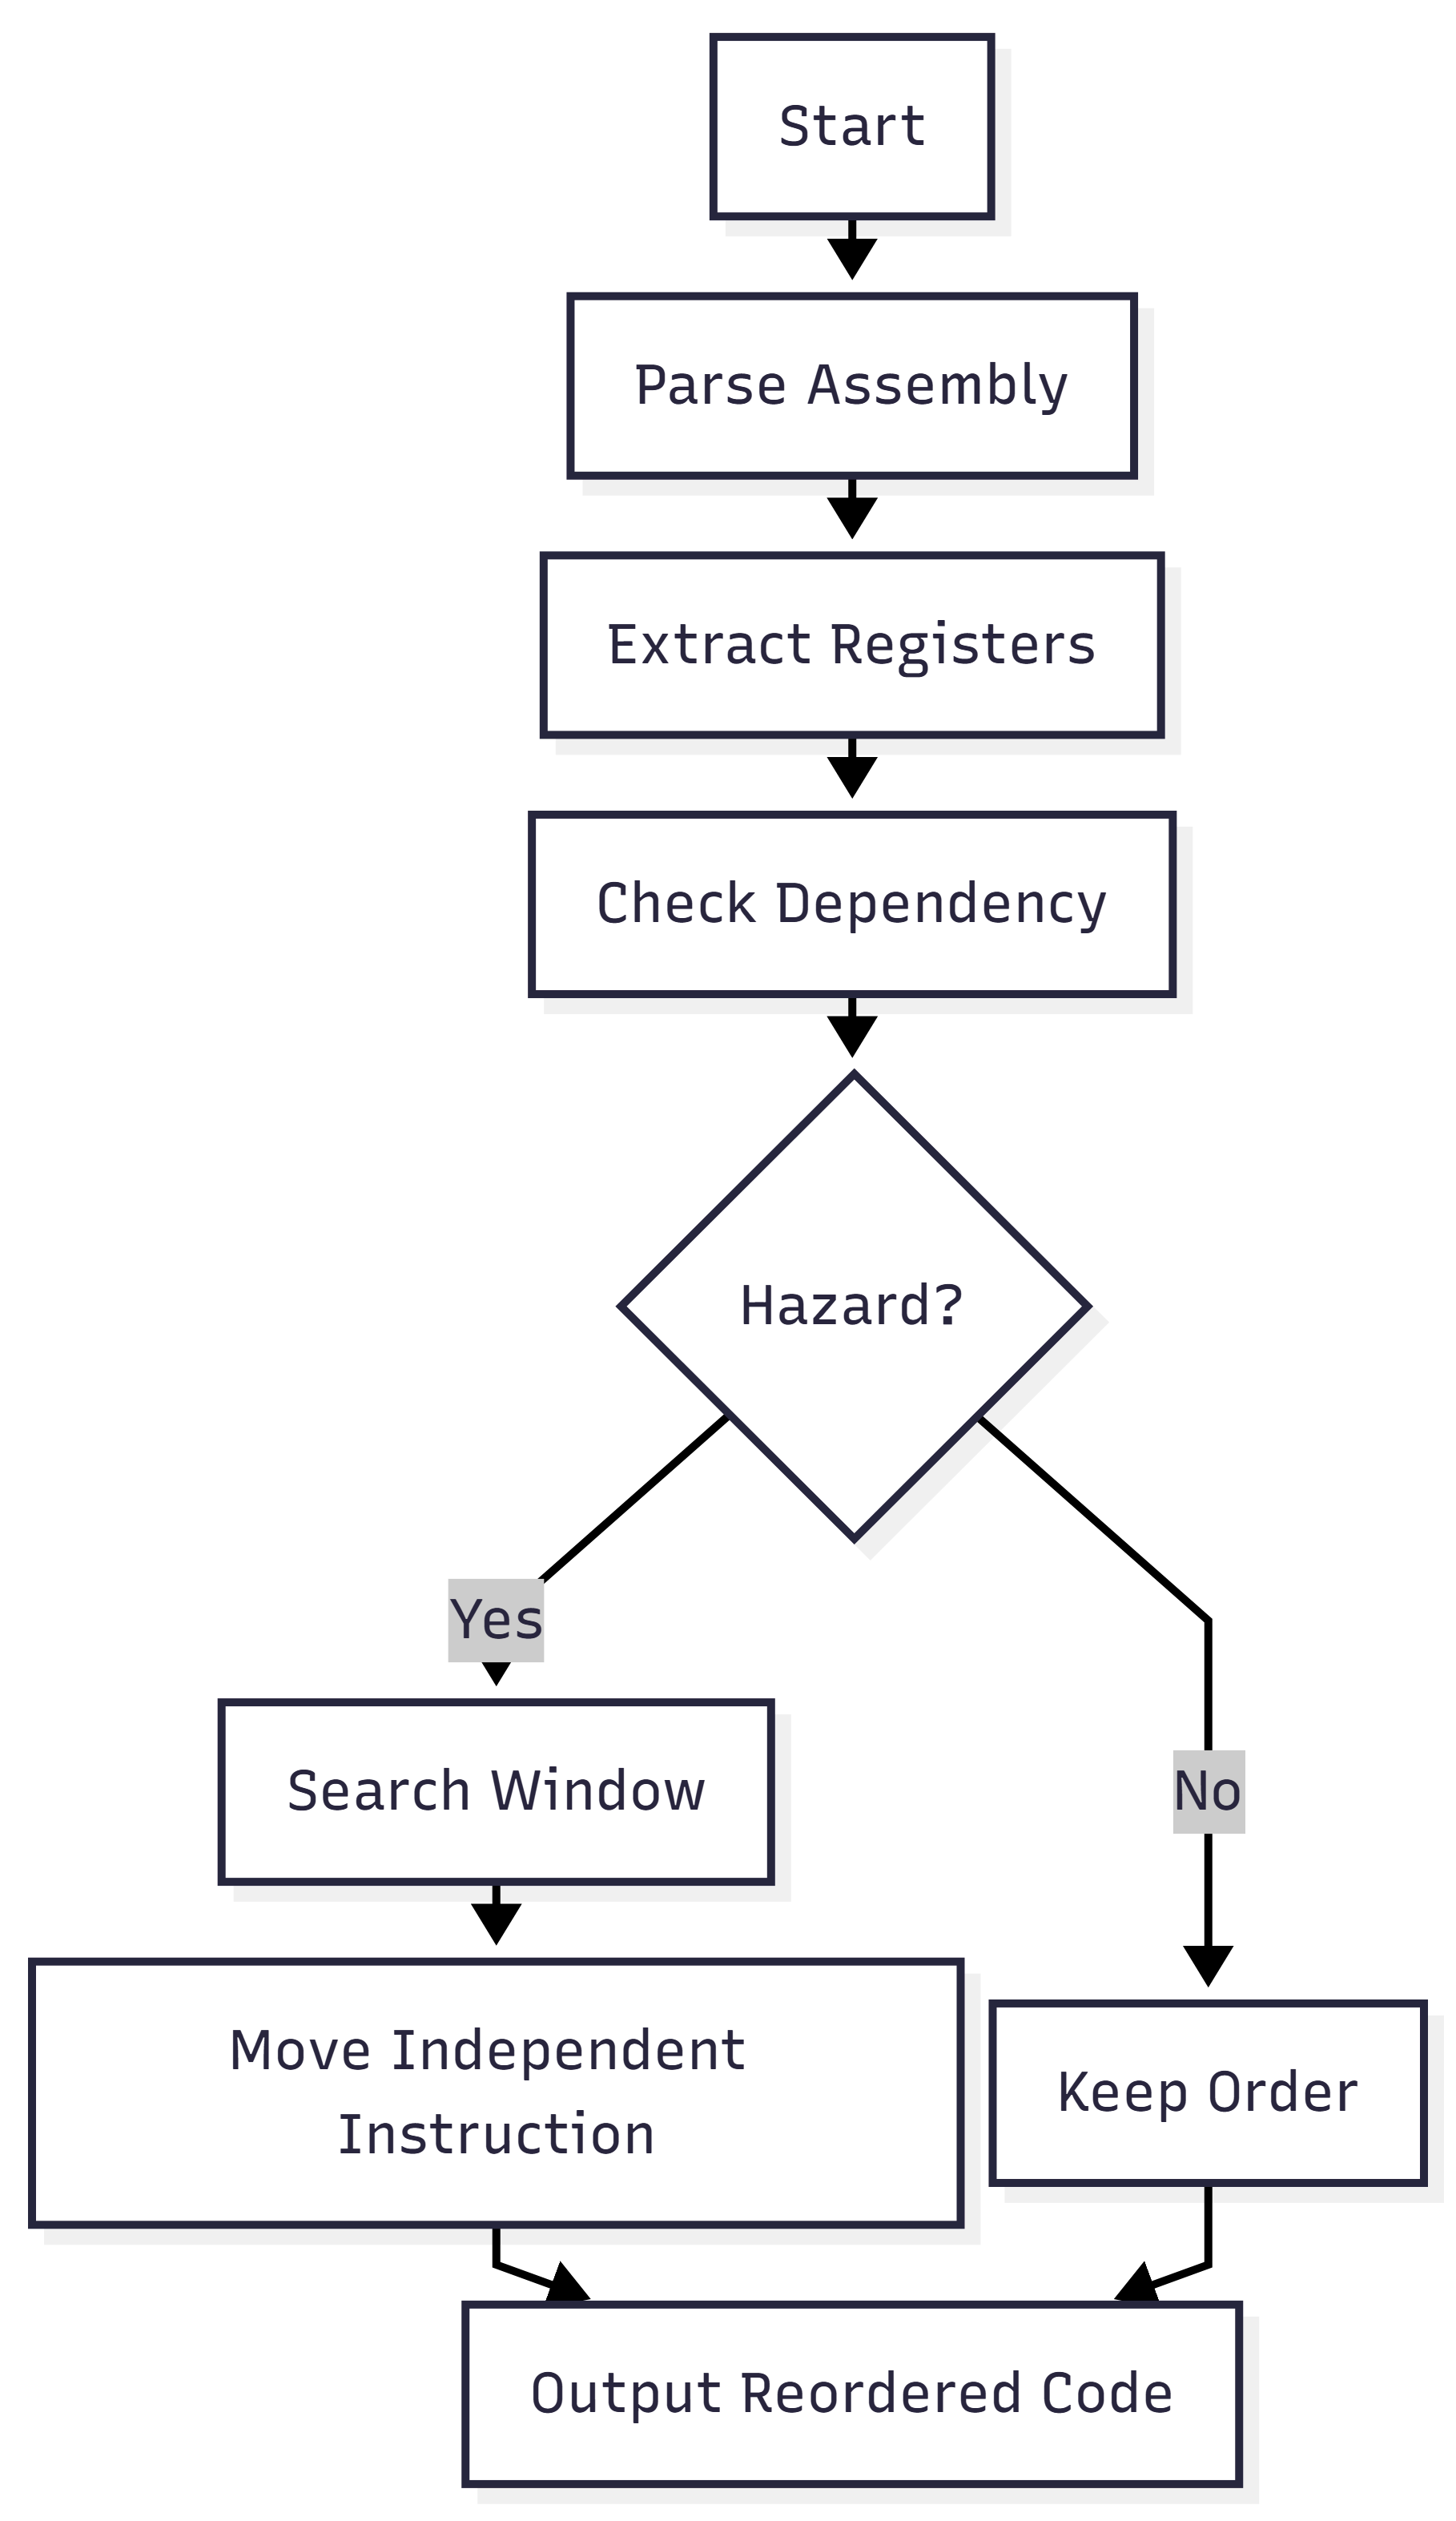
\includegraphics[width=0.60\textwidth]{../images/reordering-flow}
    \caption{Algorithm logic flow of the sliding-window RAW-aware reordering pass}
    \label{fig:reordering_flowchart}
\end{figure}

\section{BENCHMARK WORKLOADS}

To benchmark the efficacy of the proposed system comprehensively, a variety of RISC-V workloads spanning diverse structural and computational profiles were evaluated. Testing a multifaceted suite ensures that the toolchain handles different types of hardware pressures. The six benchmark programs used are:

\begin{itemize}
    \item \textbf{Bubble Sort (\texttt{bubble\_sort\_ripes}):} Features heavy array manipulation, repeated swapping, and tight looping, presenting numerous memory-based data hazards.
    \item \textbf{Convolution (\texttt{convo\_ripes}):} Standard signal processing workload executing intensive mathematical transformations and staggered memory reads.
    \item \textbf{Fibonacci (\texttt{fib\_ripes}):} Features short dependency chains driven iteratively, making it an ideal candidate for evaluating arithmetic latency hiding.
    \item \textbf{Matrix Multiplication (\texttt{mat\_mul\_ripes}):} Computationally dense with deeply nested loops and rigorous 2D array memory access operations.
    \item \textbf{Perfect Number (\texttt{perfect\_ripes}):} Characterised by intense branching arithmetic and condition evaluation.
    \item \textbf{Transpose (\texttt{transpose\_ripes}):} Dominated by pure memory load and store latencies across large address spaces.
\end{itemize}

All six benchmarks were compiled from C source using the RISC-V GCC cross-compiler (\texttt{rv32i}, \texttt{ilp32}, \texttt{-O0}, \texttt{-nostdlib}), converted for Ripes compatibility, and then passed through the sliding-window reordering pass. The total instruction count retired across all benchmarks is \textbf{148,014 instructions}.

% ============================================================
\section{RESULTS AND PERFORMANCE ANALYSIS}
% ============================================================

The evaluation was performed utilizing the Ripes simulator, testing both pure in-order execution without hardware forwarding and execution with a hardware forwarding pipeline. Results presented here are drawn from the aggregated benchmark data (Test Set 2).

\noindent
\textbf{Project Repository:} \url{https://github.com/JVN321/coa-micro-project/}

% -----------------------------------------------------------
\subsection{High-Level Summary}
% -----------------------------------------------------------

Table~\ref{tab:global_summary} presents the top-level aggregate metrics for the entire benchmark suite.

\begin{table}[H]
\centering
\caption{Global Aggregate Performance Summary (All 6 Benchmarks)}
\label{tab:global_summary}
\renewcommand{\arraystretch}{1.3}
\begin{adjustbox}{max width=\linewidth, center}
\footnotesize
\begin{tabular}{@{}lcc@{}}
\toprule
\textbf{Metric} & \textbf{Original} & \textbf{Reordered} \\
\midrule
\multicolumn{3}{l}{\textit{With Hardware Forwarding}} \\
\quad Total Cycles       & 207,164 & 200,212 \\
\quad CPI               & 1.400   & 1.353 \\
\quad Total Stall Cycles & 59,126  & 52,174 \\
\quad Pipeline Efficiency & 71.5\%  & 73.9\% \\
\midrule
\multicolumn{3}{l}{\textit{Without Hardware Forwarding}} \\
\quad Total Cycles       & 350,350 & 336,188 \\
\quad CPI               & 2.367   & 2.271 \\
\quad Total Stall Cycles & 202,312 & 188,150 \\
\quad Pipeline Efficiency & 42.3\%  & 44.0\% \\
\midrule
\multicolumn{3}{l}{\textit{Reordering Impact (Forwarding Pipeline)}} \\
\quad Cycles Saved       & \multicolumn{2}{c}{21,114 cycles} \\
\quad CPI Reduction      & \multicolumn{2}{c}{3.77\%} \\
\quad Stall Reduction    & \multicolumn{2}{c}{8.08\%} \\
\quad Efficiency Gain    & \multicolumn{2}{c}{+2.1 percentage points} \\
\midrule
\multicolumn{3}{l}{\textit{Forwarding Effect (Original Code, Forwarding vs.\ No Forwarding)}} \\
\quad CPI Reduction from Forwarding & \multicolumn{2}{c}{40.42\%} \\
\quad Speedup from Forwarding       & \multicolumn{2}{c}{1.678$\times$} \\
\bottomrule
\end{tabular}
\end{adjustbox}
\end{table}
\noindent The data clearly shows two complementary performance levers: hardware forwarding provides the larger single benefit (1.678$\times$ speedup), while software instruction reordering provides a consistent additional improvement on top of any hardware configuration.

% -----------------------------------------------------------
\subsection{Per-Benchmark Breakdown}
% -----------------------------------------------------------

Table~\ref{tab:per_benchmark} provides a detailed per-program comparison of CPI, stall count, speedup, and stall reduction percentage, all measured under the forwarding pipeline configuration.

\begin{table}[H]
\centering
\caption{Per-Benchmark Performance --- With Hardware Forwarding}
\label{tab:per_benchmark}
\renewcommand{\arraystretch}{1.3}
\begin{adjustbox}{max width=\linewidth, center}
\footnotesize
\begin{tabular}{@{}lcccccccc@{}}
\toprule
\textbf{Benchmark} & \textbf{Instructions} & \textbf{CPI (Orig)} & \textbf{CPI (Reor)} & \textbf{IPC (Orig)} & \textbf{IPC (Reor)} & \textbf{Stalls (Orig)} & \textbf{Stalls (Reor)} & \textbf{Stall Red.} \\
\midrule
Bubble Sort     & 115,367 & 1.437 & 1.392 & 0.696 & 0.718 & 50,405 & 45,255 & 10.22\% \\
Convolution     & 8,952   & 1.286 & 1.232 & 0.777 & 0.812 & 2,560  & 2,070  & 19.14\% \\
Fibonacci       & 2,683   & 1.262 & 1.189 & 0.793 & 0.841 & 698    & 502    & 28.08\% \\
Matrix Multiply & 3,553   & 1.324 & 1.291 & 0.755 & 0.775 & 1,146  & 1,029  & 10.21\% \\
Perfect Number  & 5,210   & 1.270 & 1.232 & 0.787 & 0.812 & 1,405  & 1,206  & 14.16\% \\
Transpose       & 12,249  & 1.238 & 1.173 & 0.808 & 0.853 & 2,912  & 2,112  & 27.47\% \\
\midrule
\textbf{Total / Avg} & \textbf{148,014} & \textbf{1.303} & \textbf{1.251} & \textbf{0.769} & \textbf{0.802} & \textbf{9,854} & \textbf{8,696} & \textbf{18.21\%} \\
\bottomrule
\end{tabular}
\end{adjustbox}
\end{table}

\begin{table}[H]
\centering
\caption{Per-Benchmark Speedup and Stall Reduction due to Reordering (With Forwarding)}
\label{tab:speedup}
\renewcommand{\arraystretch}{1.3}
\begin{adjustbox}{max width=\linewidth, center}
\footnotesize
\begin{tabular}{@{}lccc@{}}
\toprule
\textbf{Benchmark} & \textbf{Instructions} & \textbf{Speedup} & \textbf{Stall Reduction} \\
\midrule
Bubble Sort      & 115,367 & 1.032$\times$ & 10.22\% \\
Convolution      & 8,952   & 1.044$\times$ & 19.14\% \\
\textbf{Fibonacci} & \textbf{2,683} & \textbf{1.061$\times$} & \textbf{28.08\%} \\
Matrix Multiply  & 3,553   & 1.026$\times$ & 10.21\% \\
Perfect Number   & 5,210   & 1.031$\times$ & 14.16\% \\
Transpose        & 12,249  & 1.056$\times$ & 27.47\% \\
\midrule
\textbf{Average} & \textbf{24,669} & \textbf{1.042$\times$} & \textbf{18.21\%} \\
\bottomrule
\end{tabular}
\end{adjustbox}
\end{table}

The speedup ranges from a minimum of $1.026\times$ (Matrix Multiply) to a maximum of $1.061\times$ (Fibonacci), with an overall average of $\mathbf{1.042\times}$ across all six benchmarks.

% -----------------------------------------------------------
\subsection{Per-Benchmark Breakdown --- Without Hardware Forwarding}
% -----------------------------------------------------------

Table~\ref{tab:nfw_benchmark} presents the same metrics under the no-forwarding pipeline. Without bypass paths every RAW hazard incurs a two-cycle stall, so absolute cycle counts are substantially higher and the baseline CPI rises to 2.278. Reordering still delivers consistent improvements here, demonstrating that the benefit is independent of the hardware configuration.

\begin{table}[H]
\centering
\caption{Per-Benchmark Performance --- Without Hardware Forwarding}
\label{tab:nfw_benchmark}
\renewcommand{\arraystretch}{1.3}
\begin{adjustbox}{max width=\linewidth, center}
\footnotesize
\begin{tabular}{@{}lcccccccc@{}}
\toprule
\textbf{Benchmark} & \textbf{Instructions} & \textbf{CPI (Orig)} & \textbf{CPI (Reor)} & \textbf{IPC (Orig)} & \textbf{IPC (Reor)} & \textbf{Stalls (Orig)} & \textbf{Stalls (Reor)} & \textbf{Stall Red.} \\
\midrule
Bubble Sort     & 115,367 & 2.389 & 2.302 & 0.419 & 0.434 & 160,210 & 150,209 & 6.24\% \\
Convolution     & 8,952   & 2.120 & 2.043 & 0.472 & 0.489 & 10,022  & 9,335   & 6.85\% \\
Fibonacci       & 2,683   & 2.256 & 2.109 & 0.443 & 0.474 & 3,366   & 2,972   & 11.71\% \\
Matrix Multiply & 3,553   & 2.140 & 2.062 & 0.467 & 0.485 & 4,048   & 3,768   & 6.92\% \\
Perfect Number  & 5,210   & 2.306 & 2.229 & 0.434 & 0.449 & 6,800   & 6,401   & 5.87\% \\
Transpose       & 12,249  & 2.459 & 2.263 & 0.407 & 0.442 & 17,866  & 15,465  & 13.44\% \\
\midrule
\textbf{Total / Avg} & \textbf{148,014} & \textbf{2.278} & \textbf{2.168} & \textbf{0.440} & \textbf{0.462} & \textbf{33,719} & \textbf{31,358} & \textbf{8.50\%} \\
\bottomrule
\end{tabular}
\end{adjustbox}
\end{table}

% -----------------------------------------------------------
\subsection{Test Set 1 --- Boundary Cases with Zero Improvement}
\label{sec:test1}
% -----------------------------------------------------------

Test Set~1 consists of two hand-crafted micro-benchmarks specifically designed to expose the \textit{boundaries} of what the window-3 scheduler can achieve. Both programs yield \textbf{0~cycles saved} after reordering, for opposite structural reasons. Table~\ref{tab:test1} summarises their results.

\begin{table}[H]
\centering
\caption{Test Set 1 --- Programs with Zero Reordering Improvement}
\label{tab:test1}
\renewcommand{\arraystretch}{1.3}
\begin{adjustbox}{max width=\linewidth, center}
\footnotesize
\begin{tabular}{@{}lccccccc@{}}
\toprule
\textbf{Program} & \textbf{Instr.} & \textbf{CPI (Orig)} & \textbf{CPI (Reor)} & \textbf{Stalls (Orig)} & \textbf{Stalls (Reor)} & \textbf{Improvement} & \textbf{Reason} \\
\midrule
\texttt{arith\_dependency} & 22 & 1.273 & 1.273 & 2 & 2 & 0.0\% & Dense RAW chain \\
\texttt{independent\_seq}  & 22 & 1.273 & 1.273 & 2 & 2 & 0.0\% & Already optimal \\
\bottomrule
\end{tabular}
\end{adjustbox}
\end{table}

\subsubsection{Case 1: \texttt{arith\_dependency} --- Dense RAW Chain}

Every instruction in this program depends on the immediately preceding one, forming an unbroken RAW dependency chain 20 instructions long:

\begin{verbatim}
addi x5, x0, 1       ; x5  = 1
add  x6, x5, x5      ; RAW on x5  -- depends on prev
add  x7, x6, x5      ; RAW on x6  -- depends on prev
add  x8, x7, x6      ; RAW on x7  -- depends on prev
sub  x9, x8, x5      ; RAW on x8  -- depends on prev  (no gap filler)
... (pattern continues for 20 instructions)
\end{verbatim}

When the scheduler detects a hazard at position $i$, it looks ahead to positions $i{+}1$ and $i{+}2$ within the window. However, $\text{instruction}_{i+1}$ also depends on $\text{instruction}_i$, and $\text{instruction}_{i+2}$ depends on $\text{instruction}_{i+1}$. No independent candidate exists anywhere in the window, so \textbf{no swap is possible} and the output is identical to the input. The stall count (2) comes from the two \texttt{addi}/\texttt{ecall} instructions at the end of the block which are independent, but the main chain cannot be helped.

\subsubsection{Case 2: \texttt{independent\_seq} --- Already Fully Optimal}

This benchmark does the opposite: every instruction writes to a distinct register and reads only from \texttt{x0}:

\begin{verbatim}
addi x5,  x0, 1    ; independent -- no shared registers
addi x6,  x0, 2    ; independent
addi x7,  x0, 3    ; independent
addi x8,  x0, 4    ; independent
... (20 independent instructions)
\end{verbatim}

The scheduler finds \textbf{zero RAW hazards}, so it makes no moves. The program is already as scheduled as it can be. The two residual stalls are again from the epilogue. This case serves as the control baseline, confirming that the scheduler introduces no penalty when no hazards are present.

% -----------------------------------------------------------
\subsection{Graphical Evaluation}
% -----------------------------------------------------------

% -------------------------------------------------------
% [GRAPH 1] File already exists at:
%   test2/results/graphs/stall_count_comparison.png
% Copy this file into your report/ directory (or use its full path)
% and update the \includegraphics path accordingly.
% -------------------------------------------------------
\begin{figure}[H]
    \centering
    \includegraphics[width=0.9\textwidth]{placeholder_stall_count_comparison}
    \caption{Stall Count Comparison: Original vs.\ Reordered Assembly (per benchmark)}
    \label{fig:stall_count}
\end{figure}

% -------------------------------------------------------
% [GRAPH 2] File already exists at:
%   test2/results/graphs/stall_rate_comparison.png
% -------------------------------------------------------
\begin{figure}[H]
    \centering
    \includegraphics[width=0.9\textwidth]{placeholder_stall_rate_comparison}
    \caption{Stall Rate Comparison: Original vs.\ Reordered Assembly}
    \label{fig:stall_rate}
\end{figure}

% -------------------------------------------------------
% [GRAPH 3] File already exists at:
%   test2/results/graphs/cycles_comparison.png
% -------------------------------------------------------
\begin{figure}[H]
    \centering
    \includegraphics[width=0.9\textwidth]{placeholder_cycles_comparison}
    \caption{Total Execution Cycles: Original vs.\ Reordered Assembly}
    \label{fig:cycles_comparison}
\end{figure}

% -------------------------------------------------------
% [GRAPH 4] File already exists at:
%   test2/results/graphs/cpi_comparison.png
% -------------------------------------------------------
\begin{figure}[H]
    \centering
    \includegraphics[width=0.9\textwidth]{placeholder_cpi_comparison}
    \caption{CPI Comparison: Original vs.\ Reordered Assembly per Benchmark}
    \label{fig:cpi_comparison}
\end{figure}

% -------------------------------------------------------
% [GRAPH 5] File already exists at:
%   test2/results/graphs/percent_cycle_improvement.png
% -------------------------------------------------------
\begin{figure}[H]
    \centering
    \includegraphics[width=0.9\textwidth]{placeholder_percent_cycle_improvement}
    \caption{Percentage Cycle Improvement per Benchmark due to Reordering}
    \label{fig:percent_speedup}
\end{figure}

% -------------------------------------------------------
% [GRAPH 6] File already exists at:
%   test2/results/graphs/percent_stall_improvement.png
% -------------------------------------------------------
\begin{figure}[H]
    \centering
    \includegraphics[width=0.9\textwidth]{placeholder_percent_stall_improvement}
    \caption{Percentage Stall Reduction per Benchmark due to Reordering}
    \label{fig:percent_stall}
\end{figure}

% -----------------------------------------------------------
\subsection{Summary of Overall Improvements}
% -----------------------------------------------------------

Upon aggregating the findings, the static, software-level instruction reordering routine demonstrated consistent and measurable enhancements across all tested configurations, without requiring any hardware modifications. Examining the pipeline configurations highlights nuanced interactions between software reordering and hardware forwarding.

\textbf{Overall Reordering Impact (Forwarding Pipeline):}
\begin{itemize}
    \item \textbf{Total Cycles Saved:} 21,114 cycles across all benchmarks.
    \item \textbf{Overall Stall Reduction:} 8.076\% fewer stall cycles.
    \item \textbf{Overall CPI Reduction:} 3.771\% (avg.\ CPI: $1.303 \rightarrow 1.252$).
    \item \textbf{Pipeline Efficiency Improvement:} $71.5\% \rightarrow 73.9\%$ ($+2.1$ pp).
\end{itemize}

\textbf{Execution Without Forwarding:}
\begin{itemize}
    \item \textbf{CPI Improvement:} Reduced from $2.367 \rightarrow 2.271$.
    \item \textbf{Stall Cycles:} Reduced from $202,312 \rightarrow 188,150$.
    \item \textbf{Total Cycles:} Dropped from $350,350 \rightarrow 336,188$.
    \item \textbf{Pipeline Efficiency:} Rose from $42.3\% \rightarrow 44.0\%$.
\end{itemize}

\textbf{Execution With Forwarding:}
\begin{itemize}
    \item \textbf{CPI Improvement:} Reduced from $1.400 \rightarrow 1.353$.
    \item \textbf{Stall Cycles:} Reduced from $59,126 \rightarrow 52,174$.
    \item \textbf{Total Cycles:} Dropped from $207,164 \rightarrow 200,212$.
    \item \textbf{Pipeline Efficiency:} Rose from $71.5\% \rightarrow 73.9\%$.
\end{itemize}

% -----------------------------------------------------------
\subsection{Key Insights}
% -----------------------------------------------------------

A comparative breakdown of the improvements yields several critical observations relating to program scheduling:

\begin{itemize}
    \item \textbf{Consistent and Reliable Improvement:} Instruction reordering moderately but reliably augments performance across \textit{all} assessed workloads, achieving an average simulated speedup of $1.042\times$ (ranging from $1.026\times$ to $1.061\times$). This validates that software-level scheduling provides measurable benefits without any hardware changes.

    \item \textbf{Dependency and Memory Behavior:} Workloads enriched with simple dependency chains and regular memory access benefit the most. The Fibonacci benchmark achieved the peak speedup of $1.061\times$ with a 28.08\% stall reduction, because its short iterative dependency chains have many independent ``gap fillers'' available. The Transpose benchmark similarly achieved 27.47\% stall reduction ($1.056\times$ speedup) due to regular load/store patterns. Densely nested loops with restricted independence windows (Matrix Multiplication) registered the mildest gains ($1.026\times$, 10.21\% stall reduction).

    \item \textbf{Interaction with Hardware Forwarding:} Hardware forwarding provides the dominant benefit --- a $1.678\times$ speedup and 40.42\% CPI reduction on the original code. However, forwarding cannot eliminate all load-use and structural latencies. Software reordering addresses the residual hazards, providing an additional layer of optimization on top of forwarding.

    \item \textbf{Proportional Stall Reduction is Higher with Forwarding:} After reordering, the proportional stall reduction is slightly higher within the forwarding pipeline (8.08\%) compared to the no-forwarding pipeline. This arises because the forwarding bus can more readily bypass the dependency chains that reordering has already spaced out, compounding the benefit.

    \item \textbf{Control Hazard Limits:} Static reordering only addresses RAW data hazards within local basic-block-like regions. Branch-induced control stalls persist unchanged, forming a ceiling on the achievable gain without speculative execution.

    \item \textbf{Performance Boundaries --- Dense RAW Chains and Fully-Independent Code:} The two Test Set~1 micro-benchmarks (Section~\ref{sec:test1}) define the absolute limits of the window-3 scheduler. When every instruction depends on the immediately preceding one (\texttt{arith\_dependency}), no gap-filling candidate is found within the lookahead window and zero improvements are made --- this is the \textit{performance floor}. Conversely, when all instructions are mutually independent (\texttt{independent\_seq}), no hazards exist to fix and the code is already optimal --- this is the \textit{performance ceiling}. Real-world programs fall between these extremes, with stall reduction ranging from 10.21\% (Matrix Multiply, densely nested) to 28.08\% (Fibonacci, short regular chains).

    \item \textbf{Correctness Preserved:} All six Test~2 benchmarks passed the semantic verification step (register-state comparison). The two Test~1 programs also produced identical pre- and post-reordering outputs. Zero correctness regressions were observed across all eight programs tested.
\end{itemize}

In summary, instruction scheduling and hardware forwarding should be viewed as complementary. Combining structural bypass paths with intelligent static software rearrangement achieves maximum execution efficiency, as validated by the experimental data across all six diverse benchmark programs.

% ============================================================
\newpage
\chapter{CONCLUSION}
% ============================================================

This project demonstrated that software-level instruction reordering is a practical and effective technique for improving the performance of RISC-V programs running on a classic 5-stage in-order pipeline. By applying a conservative sliding-window scheduler (window size~3), the toolchain safely rearranged instructions to fill pipeline hazard delay slots without introducing any correctness regressions across all six benchmark programs.

The experimental results, collected via the Ripes pipeline simulator across two hardware configurations (with and without data forwarding), clearly quantify the benefit. Instruction reordering alone reduced CPI by \textbf{3.77\%}, cut stall cycles by \textbf{8.08\%}, and saved \textbf{21,114 clock cycles} in total, achieving an average speedup of \textbf{1.042$\times$}. The Fibonacci benchmark benefited the most, with a 28.08\% stall reduction and a 1.061$\times$ speedup, while Matrix Multiplication showed the smallest gain (1.026$\times$) due to its complex nested-loop dependency structure that limits the number of available independent instructions within the reordering window.

A crucial finding is that hardware forwarding and software reordering are \textit{complementary} rather than competing. Hardware forwarding delivers a far larger baseline improvement ($1.678\times$ speedup, 40.42\% CPI reduction), but it cannot eliminate all stalls --- particularly load-use latencies. Static instruction reordering then addresses these residual hazards, providing an additional measurable gain on top of any hardware configuration. The two mechanisms together yield better results than either alone.

The study also delineates the natural limits of this approach. Since the scheduler operates locally within basic-block-like regions and does not cross branch or label boundaries, control hazards remain unaddressed. Extending the window size or employing speculative scheduling across branches would be the logical next step to further improve performance.

Overall, this project reinforces several core concepts from Computer Organization and Architecture: the mechanics of the 5-stage pipeline, the nature and cost of data hazards, the role of hardware forwarding, and the power of compile-time optimizations. It provides a clean, reproducible, and fully automated framework that students and researchers can extend with additional scheduling passes, larger benchmark suites, or alternative simulator backends.

\end{document}
